\documentclass[11pt]{article}

    \usepackage[breakable]{tcolorbox}
    \usepackage{parskip} % Stop auto-indenting (to mimic markdown behaviour)
    

    % Basic figure setup, for now with no caption control since it's done
    % automatically by Pandoc (which extracts ![](path) syntax from Markdown).
    \usepackage{graphicx}
    % Keep aspect ratio if custom image width or height is specified
    \setkeys{Gin}{keepaspectratio}
    % Maintain compatibility with old templates. Remove in nbconvert 6.0
    \let\Oldincludegraphics\includegraphics
    % Ensure that by default, figures have no caption (until we provide a
    % proper Figure object with a Caption API and a way to capture that
    % in the conversion process - todo).
    \usepackage{caption}
    \DeclareCaptionFormat{nocaption}{}
    \captionsetup{format=nocaption,aboveskip=0pt,belowskip=0pt}

    \usepackage{float}
    \floatplacement{figure}{H} % forces figures to be placed at the correct location
    \usepackage{xcolor} % Allow colors to be defined
    \usepackage{enumerate} % Needed for markdown enumerations to work
    \usepackage{geometry} % Used to adjust the document margins
    \usepackage{amsmath} % Equations
    \usepackage{amssymb} % Equations
    \usepackage{textcomp} % defines textquotesingle
    % Hack from http://tex.stackexchange.com/a/47451/13684:
    \AtBeginDocument{%
        \def\PYZsq{\textquotesingle}% Upright quotes in Pygmentized code
    }
    \usepackage{upquote} % Upright quotes for verbatim code
    \usepackage{eurosym} % defines \euro

    \usepackage{iftex}
    \ifPDFTeX
        \usepackage[T1]{fontenc}
        \IfFileExists{alphabeta.sty}{
              \usepackage{alphabeta}
          }{
              \usepackage[mathletters]{ucs}
              \usepackage[utf8x]{inputenc}
          }
    \else
        \usepackage{fontspec}
        \usepackage{unicode-math}
    \fi

    \usepackage{fancyvrb} % verbatim replacement that allows latex
    \usepackage{grffile} % extends the file name processing of package graphics
                         % to support a larger range
    \makeatletter % fix for old versions of grffile with XeLaTeX
    \@ifpackagelater{grffile}{2019/11/01}
    {
      % Do nothing on new versions
    }
    {
      \def\Gread@@xetex#1{%
        \IfFileExists{"\Gin@base".bb}%
        {\Gread@eps{\Gin@base.bb}}%
        {\Gread@@xetex@aux#1}%
      }
    }
    \makeatother
    \usepackage[Export]{adjustbox} % Used to constrain images to a maximum size
    \adjustboxset{max size={0.9\linewidth}{0.9\paperheight}}

    % The hyperref package gives us a pdf with properly built
    % internal navigation ('pdf bookmarks' for the table of contents,
    % internal cross-reference links, web links for URLs, etc.)
    \usepackage{hyperref}
    % The default LaTeX title has an obnoxious amount of whitespace. By default,
    % titling removes some of it. It also provides customization options.
    \usepackage{titling}
    \usepackage{longtable} % longtable support required by pandoc >1.10
    \usepackage{booktabs}  % table support for pandoc > 1.12.2
    \usepackage{array}     % table support for pandoc >= 2.11.3
    \usepackage{calc}      % table minipage width calculation for pandoc >= 2.11.1
    \usepackage[inline]{enumitem} % IRkernel/repr support (it uses the enumerate* environment)
    \usepackage[normalem]{ulem} % ulem is needed to support strikethroughs (\sout)
                                % normalem makes italics be italics, not underlines
    \usepackage{soul}      % strikethrough (\st) support for pandoc >= 3.0.0
    \usepackage{mathrsfs}
    

    
    % Colors for the hyperref package
    \definecolor{urlcolor}{rgb}{0,.145,.698}
    \definecolor{linkcolor}{rgb}{.71,0.21,0.01}
    \definecolor{citecolor}{rgb}{.12,.54,.11}

    % ANSI colors
    \definecolor{ansi-black}{HTML}{3E424D}
    \definecolor{ansi-black-intense}{HTML}{282C36}
    \definecolor{ansi-red}{HTML}{E75C58}
    \definecolor{ansi-red-intense}{HTML}{B22B31}
    \definecolor{ansi-green}{HTML}{00A250}
    \definecolor{ansi-green-intense}{HTML}{007427}
    \definecolor{ansi-yellow}{HTML}{DDB62B}
    \definecolor{ansi-yellow-intense}{HTML}{B27D12}
    \definecolor{ansi-blue}{HTML}{208FFB}
    \definecolor{ansi-blue-intense}{HTML}{0065CA}
    \definecolor{ansi-magenta}{HTML}{D160C4}
    \definecolor{ansi-magenta-intense}{HTML}{A03196}
    \definecolor{ansi-cyan}{HTML}{60C6C8}
    \definecolor{ansi-cyan-intense}{HTML}{258F8F}
    \definecolor{ansi-white}{HTML}{C5C1B4}
    \definecolor{ansi-white-intense}{HTML}{A1A6B2}
    \definecolor{ansi-default-inverse-fg}{HTML}{FFFFFF}
    \definecolor{ansi-default-inverse-bg}{HTML}{000000}

    % common color for the border for error outputs.
    \definecolor{outerrorbackground}{HTML}{FFDFDF}

    % commands and environments needed by pandoc snippets
    % extracted from the output of `pandoc -s`
    \providecommand{\tightlist}{%
      \setlength{\itemsep}{0pt}\setlength{\parskip}{0pt}}
    \DefineVerbatimEnvironment{Highlighting}{Verbatim}{commandchars=\\\{\}}
    % Add ',fontsize=\small' for more characters per line
    \newenvironment{Shaded}{}{}
    \newcommand{\KeywordTok}[1]{\textcolor[rgb]{0.00,0.44,0.13}{\textbf{{#1}}}}
    \newcommand{\DataTypeTok}[1]{\textcolor[rgb]{0.56,0.13,0.00}{{#1}}}
    \newcommand{\DecValTok}[1]{\textcolor[rgb]{0.25,0.63,0.44}{{#1}}}
    \newcommand{\BaseNTok}[1]{\textcolor[rgb]{0.25,0.63,0.44}{{#1}}}
    \newcommand{\FloatTok}[1]{\textcolor[rgb]{0.25,0.63,0.44}{{#1}}}
    \newcommand{\CharTok}[1]{\textcolor[rgb]{0.25,0.44,0.63}{{#1}}}
    \newcommand{\StringTok}[1]{\textcolor[rgb]{0.25,0.44,0.63}{{#1}}}
    \newcommand{\CommentTok}[1]{\textcolor[rgb]{0.38,0.63,0.69}{\textit{{#1}}}}
    \newcommand{\OtherTok}[1]{\textcolor[rgb]{0.00,0.44,0.13}{{#1}}}
    \newcommand{\AlertTok}[1]{\textcolor[rgb]{1.00,0.00,0.00}{\textbf{{#1}}}}
    \newcommand{\FunctionTok}[1]{\textcolor[rgb]{0.02,0.16,0.49}{{#1}}}
    \newcommand{\RegionMarkerTok}[1]{{#1}}
    \newcommand{\ErrorTok}[1]{\textcolor[rgb]{1.00,0.00,0.00}{\textbf{{#1}}}}
    \newcommand{\NormalTok}[1]{{#1}}

    % Additional commands for more recent versions of Pandoc
    \newcommand{\ConstantTok}[1]{\textcolor[rgb]{0.53,0.00,0.00}{{#1}}}
    \newcommand{\SpecialCharTok}[1]{\textcolor[rgb]{0.25,0.44,0.63}{{#1}}}
    \newcommand{\VerbatimStringTok}[1]{\textcolor[rgb]{0.25,0.44,0.63}{{#1}}}
    \newcommand{\SpecialStringTok}[1]{\textcolor[rgb]{0.73,0.40,0.53}{{#1}}}
    \newcommand{\ImportTok}[1]{{#1}}
    \newcommand{\DocumentationTok}[1]{\textcolor[rgb]{0.73,0.13,0.13}{\textit{{#1}}}}
    \newcommand{\AnnotationTok}[1]{\textcolor[rgb]{0.38,0.63,0.69}{\textbf{\textit{{#1}}}}}
    \newcommand{\CommentVarTok}[1]{\textcolor[rgb]{0.38,0.63,0.69}{\textbf{\textit{{#1}}}}}
    \newcommand{\VariableTok}[1]{\textcolor[rgb]{0.10,0.09,0.49}{{#1}}}
    \newcommand{\ControlFlowTok}[1]{\textcolor[rgb]{0.00,0.44,0.13}{\textbf{{#1}}}}
    \newcommand{\OperatorTok}[1]{\textcolor[rgb]{0.40,0.40,0.40}{{#1}}}
    \newcommand{\BuiltInTok}[1]{{#1}}
    \newcommand{\ExtensionTok}[1]{{#1}}
    \newcommand{\PreprocessorTok}[1]{\textcolor[rgb]{0.74,0.48,0.00}{{#1}}}
    \newcommand{\AttributeTok}[1]{\textcolor[rgb]{0.49,0.56,0.16}{{#1}}}
    \newcommand{\InformationTok}[1]{\textcolor[rgb]{0.38,0.63,0.69}{\textbf{\textit{{#1}}}}}
    \newcommand{\WarningTok}[1]{\textcolor[rgb]{0.38,0.63,0.69}{\textbf{\textit{{#1}}}}}
    \makeatletter
    \newsavebox\pandoc@box
    \newcommand*\pandocbounded[1]{%
      \sbox\pandoc@box{#1}%
      % scaling factors for width and height
      \Gscale@div\@tempa\textheight{\dimexpr\ht\pandoc@box+\dp\pandoc@box\relax}%
      \Gscale@div\@tempb\linewidth{\wd\pandoc@box}%
      % select the smaller of both
      \ifdim\@tempb\p@<\@tempa\p@
        \let\@tempa\@tempb
      \fi
      % scaling accordingly (\@tempa < 1)
      \ifdim\@tempa\p@<\p@
        \scalebox{\@tempa}{\usebox\pandoc@box}%
      % scaling not needed, use as it is
      \else
        \usebox{\pandoc@box}%
      \fi
    }
    \makeatother

    % Define a nice break command that doesn't care if a line doesn't already
    % exist.
    \def\br{\hspace*{\fill} \\* }
    % Math Jax compatibility definitions
    \def\gt{>}
    \def\lt{<}
    \let\Oldtex\TeX
    \let\Oldlatex\LaTeX
    \renewcommand{\TeX}{\textrm{\Oldtex}}
    \renewcommand{\LaTeX}{\textrm{\Oldlatex}}
    % Document parameters
    % Document title
    \title{hw1}
    
    
    
    
    
    
    
% Pygments definitions
\makeatletter
\def\PY@reset{\let\PY@it=\relax \let\PY@bf=\relax%
    \let\PY@ul=\relax \let\PY@tc=\relax%
    \let\PY@bc=\relax \let\PY@ff=\relax}
\def\PY@tok#1{\csname PY@tok@#1\endcsname}
\def\PY@toks#1+{\ifx\relax#1\empty\else%
    \PY@tok{#1}\expandafter\PY@toks\fi}
\def\PY@do#1{\PY@bc{\PY@tc{\PY@ul{%
    \PY@it{\PY@bf{\PY@ff{#1}}}}}}}
\def\PY#1#2{\PY@reset\PY@toks#1+\relax+\PY@do{#2}}

\@namedef{PY@tok@w}{\def\PY@tc##1{\textcolor[rgb]{0.73,0.73,0.73}{##1}}}
\@namedef{PY@tok@c}{\let\PY@it=\textit\def\PY@tc##1{\textcolor[rgb]{0.24,0.48,0.48}{##1}}}
\@namedef{PY@tok@cp}{\def\PY@tc##1{\textcolor[rgb]{0.61,0.40,0.00}{##1}}}
\@namedef{PY@tok@k}{\let\PY@bf=\textbf\def\PY@tc##1{\textcolor[rgb]{0.00,0.50,0.00}{##1}}}
\@namedef{PY@tok@kp}{\def\PY@tc##1{\textcolor[rgb]{0.00,0.50,0.00}{##1}}}
\@namedef{PY@tok@kt}{\def\PY@tc##1{\textcolor[rgb]{0.69,0.00,0.25}{##1}}}
\@namedef{PY@tok@o}{\def\PY@tc##1{\textcolor[rgb]{0.40,0.40,0.40}{##1}}}
\@namedef{PY@tok@ow}{\let\PY@bf=\textbf\def\PY@tc##1{\textcolor[rgb]{0.67,0.13,1.00}{##1}}}
\@namedef{PY@tok@nb}{\def\PY@tc##1{\textcolor[rgb]{0.00,0.50,0.00}{##1}}}
\@namedef{PY@tok@nf}{\def\PY@tc##1{\textcolor[rgb]{0.00,0.00,1.00}{##1}}}
\@namedef{PY@tok@nc}{\let\PY@bf=\textbf\def\PY@tc##1{\textcolor[rgb]{0.00,0.00,1.00}{##1}}}
\@namedef{PY@tok@nn}{\let\PY@bf=\textbf\def\PY@tc##1{\textcolor[rgb]{0.00,0.00,1.00}{##1}}}
\@namedef{PY@tok@ne}{\let\PY@bf=\textbf\def\PY@tc##1{\textcolor[rgb]{0.80,0.25,0.22}{##1}}}
\@namedef{PY@tok@nv}{\def\PY@tc##1{\textcolor[rgb]{0.10,0.09,0.49}{##1}}}
\@namedef{PY@tok@no}{\def\PY@tc##1{\textcolor[rgb]{0.53,0.00,0.00}{##1}}}
\@namedef{PY@tok@nl}{\def\PY@tc##1{\textcolor[rgb]{0.46,0.46,0.00}{##1}}}
\@namedef{PY@tok@ni}{\let\PY@bf=\textbf\def\PY@tc##1{\textcolor[rgb]{0.44,0.44,0.44}{##1}}}
\@namedef{PY@tok@na}{\def\PY@tc##1{\textcolor[rgb]{0.41,0.47,0.13}{##1}}}
\@namedef{PY@tok@nt}{\let\PY@bf=\textbf\def\PY@tc##1{\textcolor[rgb]{0.00,0.50,0.00}{##1}}}
\@namedef{PY@tok@nd}{\def\PY@tc##1{\textcolor[rgb]{0.67,0.13,1.00}{##1}}}
\@namedef{PY@tok@s}{\def\PY@tc##1{\textcolor[rgb]{0.73,0.13,0.13}{##1}}}
\@namedef{PY@tok@sd}{\let\PY@it=\textit\def\PY@tc##1{\textcolor[rgb]{0.73,0.13,0.13}{##1}}}
\@namedef{PY@tok@si}{\let\PY@bf=\textbf\def\PY@tc##1{\textcolor[rgb]{0.64,0.35,0.47}{##1}}}
\@namedef{PY@tok@se}{\let\PY@bf=\textbf\def\PY@tc##1{\textcolor[rgb]{0.67,0.36,0.12}{##1}}}
\@namedef{PY@tok@sr}{\def\PY@tc##1{\textcolor[rgb]{0.64,0.35,0.47}{##1}}}
\@namedef{PY@tok@ss}{\def\PY@tc##1{\textcolor[rgb]{0.10,0.09,0.49}{##1}}}
\@namedef{PY@tok@sx}{\def\PY@tc##1{\textcolor[rgb]{0.00,0.50,0.00}{##1}}}
\@namedef{PY@tok@m}{\def\PY@tc##1{\textcolor[rgb]{0.40,0.40,0.40}{##1}}}
\@namedef{PY@tok@gh}{\let\PY@bf=\textbf\def\PY@tc##1{\textcolor[rgb]{0.00,0.00,0.50}{##1}}}
\@namedef{PY@tok@gu}{\let\PY@bf=\textbf\def\PY@tc##1{\textcolor[rgb]{0.50,0.00,0.50}{##1}}}
\@namedef{PY@tok@gd}{\def\PY@tc##1{\textcolor[rgb]{0.63,0.00,0.00}{##1}}}
\@namedef{PY@tok@gi}{\def\PY@tc##1{\textcolor[rgb]{0.00,0.52,0.00}{##1}}}
\@namedef{PY@tok@gr}{\def\PY@tc##1{\textcolor[rgb]{0.89,0.00,0.00}{##1}}}
\@namedef{PY@tok@ge}{\let\PY@it=\textit}
\@namedef{PY@tok@gs}{\let\PY@bf=\textbf}
\@namedef{PY@tok@ges}{\let\PY@bf=\textbf\let\PY@it=\textit}
\@namedef{PY@tok@gp}{\let\PY@bf=\textbf\def\PY@tc##1{\textcolor[rgb]{0.00,0.00,0.50}{##1}}}
\@namedef{PY@tok@go}{\def\PY@tc##1{\textcolor[rgb]{0.44,0.44,0.44}{##1}}}
\@namedef{PY@tok@gt}{\def\PY@tc##1{\textcolor[rgb]{0.00,0.27,0.87}{##1}}}
\@namedef{PY@tok@err}{\def\PY@bc##1{{\setlength{\fboxsep}{\string -\fboxrule}\fcolorbox[rgb]{1.00,0.00,0.00}{1,1,1}{\strut ##1}}}}
\@namedef{PY@tok@kc}{\let\PY@bf=\textbf\def\PY@tc##1{\textcolor[rgb]{0.00,0.50,0.00}{##1}}}
\@namedef{PY@tok@kd}{\let\PY@bf=\textbf\def\PY@tc##1{\textcolor[rgb]{0.00,0.50,0.00}{##1}}}
\@namedef{PY@tok@kn}{\let\PY@bf=\textbf\def\PY@tc##1{\textcolor[rgb]{0.00,0.50,0.00}{##1}}}
\@namedef{PY@tok@kr}{\let\PY@bf=\textbf\def\PY@tc##1{\textcolor[rgb]{0.00,0.50,0.00}{##1}}}
\@namedef{PY@tok@bp}{\def\PY@tc##1{\textcolor[rgb]{0.00,0.50,0.00}{##1}}}
\@namedef{PY@tok@fm}{\def\PY@tc##1{\textcolor[rgb]{0.00,0.00,1.00}{##1}}}
\@namedef{PY@tok@vc}{\def\PY@tc##1{\textcolor[rgb]{0.10,0.09,0.49}{##1}}}
\@namedef{PY@tok@vg}{\def\PY@tc##1{\textcolor[rgb]{0.10,0.09,0.49}{##1}}}
\@namedef{PY@tok@vi}{\def\PY@tc##1{\textcolor[rgb]{0.10,0.09,0.49}{##1}}}
\@namedef{PY@tok@vm}{\def\PY@tc##1{\textcolor[rgb]{0.10,0.09,0.49}{##1}}}
\@namedef{PY@tok@sa}{\def\PY@tc##1{\textcolor[rgb]{0.73,0.13,0.13}{##1}}}
\@namedef{PY@tok@sb}{\def\PY@tc##1{\textcolor[rgb]{0.73,0.13,0.13}{##1}}}
\@namedef{PY@tok@sc}{\def\PY@tc##1{\textcolor[rgb]{0.73,0.13,0.13}{##1}}}
\@namedef{PY@tok@dl}{\def\PY@tc##1{\textcolor[rgb]{0.73,0.13,0.13}{##1}}}
\@namedef{PY@tok@s2}{\def\PY@tc##1{\textcolor[rgb]{0.73,0.13,0.13}{##1}}}
\@namedef{PY@tok@sh}{\def\PY@tc##1{\textcolor[rgb]{0.73,0.13,0.13}{##1}}}
\@namedef{PY@tok@s1}{\def\PY@tc##1{\textcolor[rgb]{0.73,0.13,0.13}{##1}}}
\@namedef{PY@tok@mb}{\def\PY@tc##1{\textcolor[rgb]{0.40,0.40,0.40}{##1}}}
\@namedef{PY@tok@mf}{\def\PY@tc##1{\textcolor[rgb]{0.40,0.40,0.40}{##1}}}
\@namedef{PY@tok@mh}{\def\PY@tc##1{\textcolor[rgb]{0.40,0.40,0.40}{##1}}}
\@namedef{PY@tok@mi}{\def\PY@tc##1{\textcolor[rgb]{0.40,0.40,0.40}{##1}}}
\@namedef{PY@tok@il}{\def\PY@tc##1{\textcolor[rgb]{0.40,0.40,0.40}{##1}}}
\@namedef{PY@tok@mo}{\def\PY@tc##1{\textcolor[rgb]{0.40,0.40,0.40}{##1}}}
\@namedef{PY@tok@ch}{\let\PY@it=\textit\def\PY@tc##1{\textcolor[rgb]{0.24,0.48,0.48}{##1}}}
\@namedef{PY@tok@cm}{\let\PY@it=\textit\def\PY@tc##1{\textcolor[rgb]{0.24,0.48,0.48}{##1}}}
\@namedef{PY@tok@cpf}{\let\PY@it=\textit\def\PY@tc##1{\textcolor[rgb]{0.24,0.48,0.48}{##1}}}
\@namedef{PY@tok@c1}{\let\PY@it=\textit\def\PY@tc##1{\textcolor[rgb]{0.24,0.48,0.48}{##1}}}
\@namedef{PY@tok@cs}{\let\PY@it=\textit\def\PY@tc##1{\textcolor[rgb]{0.24,0.48,0.48}{##1}}}

\def\PYZbs{\char`\\}
\def\PYZus{\char`\_}
\def\PYZob{\char`\{}
\def\PYZcb{\char`\}}
\def\PYZca{\char`\^}
\def\PYZam{\char`\&}
\def\PYZlt{\char`\<}
\def\PYZgt{\char`\>}
\def\PYZsh{\char`\#}
\def\PYZpc{\char`\%}
\def\PYZdl{\char`\$}
\def\PYZhy{\char`\-}
\def\PYZsq{\char`\'}
\def\PYZdq{\char`\"}
\def\PYZti{\char`\~}
% for compatibility with earlier versions
\def\PYZat{@}
\def\PYZlb{[}
\def\PYZrb{]}
\makeatother


    % For linebreaks inside Verbatim environment from package fancyvrb.
    \makeatletter
        \newbox\Wrappedcontinuationbox
        \newbox\Wrappedvisiblespacebox
        \newcommand*\Wrappedvisiblespace {\textcolor{red}{\textvisiblespace}}
        \newcommand*\Wrappedcontinuationsymbol {\textcolor{red}{\llap{\tiny$\m@th\hookrightarrow$}}}
        \newcommand*\Wrappedcontinuationindent {3ex }
        \newcommand*\Wrappedafterbreak {\kern\Wrappedcontinuationindent\copy\Wrappedcontinuationbox}
        % Take advantage of the already applied Pygments mark-up to insert
        % potential linebreaks for TeX processing.
        %        {, <, #, %, $, ' and ": go to next line.
        %        _, }, ^, &, >, - and ~: stay at end of broken line.
        % Use of \textquotesingle for straight quote.
        \newcommand*\Wrappedbreaksatspecials {%
            \def\PYGZus{\discretionary{\char`\_}{\Wrappedafterbreak}{\char`\_}}%
            \def\PYGZob{\discretionary{}{\Wrappedafterbreak\char`\{}{\char`\{}}%
            \def\PYGZcb{\discretionary{\char`\}}{\Wrappedafterbreak}{\char`\}}}%
            \def\PYGZca{\discretionary{\char`\^}{\Wrappedafterbreak}{\char`\^}}%
            \def\PYGZam{\discretionary{\char`\&}{\Wrappedafterbreak}{\char`\&}}%
            \def\PYGZlt{\discretionary{}{\Wrappedafterbreak\char`\<}{\char`\<}}%
            \def\PYGZgt{\discretionary{\char`\>}{\Wrappedafterbreak}{\char`\>}}%
            \def\PYGZsh{\discretionary{}{\Wrappedafterbreak\char`\#}{\char`\#}}%
            \def\PYGZpc{\discretionary{}{\Wrappedafterbreak\char`\%}{\char`\%}}%
            \def\PYGZdl{\discretionary{}{\Wrappedafterbreak\char`\$}{\char`\$}}%
            \def\PYGZhy{\discretionary{\char`\-}{\Wrappedafterbreak}{\char`\-}}%
            \def\PYGZsq{\discretionary{}{\Wrappedafterbreak\textquotesingle}{\textquotesingle}}%
            \def\PYGZdq{\discretionary{}{\Wrappedafterbreak\char`\"}{\char`\"}}%
            \def\PYGZti{\discretionary{\char`\~}{\Wrappedafterbreak}{\char`\~}}%
        }
        % Some characters . , ; ? ! / are not pygmentized.
        % This macro makes them "active" and they will insert potential linebreaks
        \newcommand*\Wrappedbreaksatpunct {%
            \lccode`\~`\.\lowercase{\def~}{\discretionary{\hbox{\char`\.}}{\Wrappedafterbreak}{\hbox{\char`\.}}}%
            \lccode`\~`\,\lowercase{\def~}{\discretionary{\hbox{\char`\,}}{\Wrappedafterbreak}{\hbox{\char`\,}}}%
            \lccode`\~`\;\lowercase{\def~}{\discretionary{\hbox{\char`\;}}{\Wrappedafterbreak}{\hbox{\char`\;}}}%
            \lccode`\~`\:\lowercase{\def~}{\discretionary{\hbox{\char`\:}}{\Wrappedafterbreak}{\hbox{\char`\:}}}%
            \lccode`\~`\?\lowercase{\def~}{\discretionary{\hbox{\char`\?}}{\Wrappedafterbreak}{\hbox{\char`\?}}}%
            \lccode`\~`\!\lowercase{\def~}{\discretionary{\hbox{\char`\!}}{\Wrappedafterbreak}{\hbox{\char`\!}}}%
            \lccode`\~`\/\lowercase{\def~}{\discretionary{\hbox{\char`\/}}{\Wrappedafterbreak}{\hbox{\char`\/}}}%
            \catcode`\.\active
            \catcode`\,\active
            \catcode`\;\active
            \catcode`\:\active
            \catcode`\?\active
            \catcode`\!\active
            \catcode`\/\active
            \lccode`\~`\~
        }
    \makeatother

    \let\OriginalVerbatim=\Verbatim
    \makeatletter
    \renewcommand{\Verbatim}[1][1]{%
        %\parskip\z@skip
        \sbox\Wrappedcontinuationbox {\Wrappedcontinuationsymbol}%
        \sbox\Wrappedvisiblespacebox {\FV@SetupFont\Wrappedvisiblespace}%
        \def\FancyVerbFormatLine ##1{\hsize\linewidth
            \vtop{\raggedright\hyphenpenalty\z@\exhyphenpenalty\z@
                \doublehyphendemerits\z@\finalhyphendemerits\z@
                \strut ##1\strut}%
        }%
        % If the linebreak is at a space, the latter will be displayed as visible
        % space at end of first line, and a continuation symbol starts next line.
        % Stretch/shrink are however usually zero for typewriter font.
        \def\FV@Space {%
            \nobreak\hskip\z@ plus\fontdimen3\font minus\fontdimen4\font
            \discretionary{\copy\Wrappedvisiblespacebox}{\Wrappedafterbreak}
            {\kern\fontdimen2\font}%
        }%

        % Allow breaks at special characters using \PYG... macros.
        \Wrappedbreaksatspecials
        % Breaks at punctuation characters . , ; ? ! and / need catcode=\active
        \OriginalVerbatim[#1,codes*=\Wrappedbreaksatpunct]%
    }
    \makeatother

    % Exact colors from NB
    \definecolor{incolor}{HTML}{303F9F}
    \definecolor{outcolor}{HTML}{D84315}
    \definecolor{cellborder}{HTML}{CFCFCF}
    \definecolor{cellbackground}{HTML}{F7F7F7}

    % prompt
    \makeatletter
    \newcommand{\boxspacing}{\kern\kvtcb@left@rule\kern\kvtcb@boxsep}
    \makeatother
    \newcommand{\prompt}[4]{
        {\ttfamily\llap{{\color{#2}[#3]:\hspace{3pt}#4}}\vspace{-\baselineskip}}
    }
    

    
    % Prevent overflowing lines due to hard-to-break entities
    \sloppy
    % Setup hyperref package
    \hypersetup{
      breaklinks=true,  % so long urls are correctly broken across lines
      colorlinks=true,
      urlcolor=urlcolor,
      linkcolor=linkcolor,
      citecolor=citecolor,
      }
    % Slightly bigger margins than the latex defaults
    
    \geometry{verbose,tmargin=1in,bmargin=1in,lmargin=1in,rmargin=1in}
    
    

\begin{document}
    
    \maketitle
    
    

    
    \section{Homework 1 (Due 24 Jan)}\label{homework-1-due-24-jan}

\textbf{Due January 24 (midnight)}

Date: \textbf{Jan 8, 2024} Total points: \textbf{100}.

    \textbf{Practicalities about homeworks and projects}

\begin{enumerate}
\def\labelenumi{\arabic{enumi}.}
\tightlist
\item
  You can work in groups (optimal groups are often 2-3 people) or by
  yourself. If you work as a group you can hand in one answer only if
  you wish. \textbf{Remember to write your name(s)}!
\item
  Homeworks are available approximately ten days before the deadline.
  You should anticipate this work.
\item
  How do I(we) hand in? You can hand in the paper and pencil exercises
  as a \textbf{single scanned PDF document}. For this homework this
  applies to exercises 1-5. Your jupyter notebook file should be
  converted to a \textbf{PDF} file, attached to the same PDF file as for
  the pencil and paper exercises. All files should be uploaded to
  Gradescope.
\end{enumerate}

\textbf{\href{../resources/gradescope-submissions.md}{Instructions for
submitting to Gradescope}.}

    \subsection{Exercise 1 (15 pt), math reminder, properties of exponential
function}\label{exercise-1-15-pt-math-reminder-properties-of-exponential-function}

The first exercise is meant to remind ourselves about properties of the
exponential function and imaginary numbers. This is highly relevant
later in this course when we start analyzing oscillatory motion and some
wave mechanics. The discovery relating
\href{https://en.wikipedia.org/wiki/Euler's_formula}{trigonometric
functions and exponential functions} is attributed to
\href{https://en.wikipedia.org/wiki/Leonhard_Euler}{Leonhard Euler
(1707-1783)}. There's two great books on the development formula, its
importance to math and science, its applications:

\begin{itemize}
\tightlist
\item
  \href{https://bookshop.org/p/books/dr-euler-s-fabulous-formula-cures-many-mathematical-ills-paul-j-nahin/9008263}{Paul
  J. Nahin, \emph{Dr.~Euler's Fabulous Formula: Cures Many Mathematical
  Ills}, Princeton University Press (2006)}
\item
  \href{https://bookshop.org/p/books/a-most-elegant-equation-euler-s-formula-and-the-beauty-of-mathematics-david-stipp/11457298}{David
  Stipp, \emph{A Most Elegant Equation: Euler's Formula and the Beauty
  of Mathematics}, Basic Books (2017)}
\end{itemize}

As physicists we should feel comfortable with expressions that include
\(\exp{(\imath \omega t)}\) and \(\exp{(\imath 2\pi f t)}\). Here \(t\)
could be interpreted as time and \(\omega\)/\(f\) as a frequency. We
know that \(\imath = \sqrt(-1)\) is the imaginary unit number.

\begin{itemize}
\tightlist
\item
  1a (4pt): Perform Taylor expansions in powers of \(2\pi f t\) of the
  functions \(\cos{(2\pi f t)}\) and \(\sin{(2\pi f t)}\). Show your
  work in producing those Taylor expansions.
\item
  1b (3pt): Perform a Taylor expansion of \(\exp{(i2\pi f t)}\). Show
  your work in producing those Taylor expansions.
\item
  1c (2pt): Using parts (a) and (b) here, show that
  \(\exp{(\imath2\pi f t)}=\cos{(2\pi f t)}+\imath\sin{(2\pi f t)}\).
\item
  1d (2pt): Show that \(\ln{(-1)} = \imath\pi\).
\item
  1e (4pt): Develop another novel mathematical relationship based on the
  properties you've discovered in this problem. Explain how your result
  connects to any of the results parts a-d.
\end{itemize}

    \subsection{Exercise 2 (15 pt), Vector
algebra}\label{exercise-2-15-pt-vector-algebra}

As we have quickly realized, forces and motion in three dimensions are
best described using vectors. Here we perform some elementary vector
algebra that we wil need to have as tacit knowledge for the rest of the
course. These operations are not typically taken with specific numbers,
but rather with vectors in general. When we need to, we use the notation
\(\boldsymbol{a}=(a_x,a_y,a_z)\) for vectors in three dimensions. To get
us started the first two questions below include numerical values, but
the third question expects you to use the general notation.

\begin{itemize}
\item
  2a (4pt) One of the many uses of the scalar product is to find the
  angle between two given vectors. Find the angle between the vectors
  \(\boldsymbol{a}=(1,3,9)\) and \(\boldsymbol{b}=(9,3,1)\) by
  evaluating their scalar product.
\item
  2b (5pt) For a cube with sides of length 1, one vertex at the origin,
  and sides along the \(x\), \(y\), and \(z\) axes, the vector of the
  body diagonal from the origin can be written
  \(\boldsymbol{a}=(1, 1, 1)\) and the vector of the face diagonal in
  the \(xy\) plane from the origin is \(\boldsymbol{b}=(1,1,0)\). Find
  first the lengths of the body diagonal and the face diagonal. Use then
  part (2a) to find the angle between the body diagonal and the face
  diagonal. \textbf{Make sure to include a sketch of your cube, the
  relevant vectors, and the angle you find.}
\item
  2c (6pt) Consider two arbitrary vectors in three dimensions,
  \(\boldsymbol{a}=(a_x, a_y, a_z)\) and
  \(\boldsymbol{b}=(b_x, b_y, b_z)\). Prove that the cross product
  \(\boldsymbol{a} \times \boldsymbol{b}\) results in a vector that is
  perpendicular to both \(\boldsymbol{a}\) and \(\boldsymbol{b}\). Use
  the properties of the dot product and the cross product to support
  your proof. Include a diagram illustrating the vectors and their cross
  product.
\end{itemize}

The notation that we use for vectors in fairly recently developed in
mathematical history. The development of calculus, geometry, and physics
in the 17th century required new notations. The
\href{https://en.wikipedia.org/wiki/History_of_mathematical_notation\#High_division_operators_and_functions}{history
of mathematical notation} is very interesting in that these tools and
symbols that we developed helped us to solve new and more advanced
problems.

    \subsection{Exercise 3 (10 pt), More vector
mathematics}\label{exercise-3-10-pt-more-vector-mathematics}

\begin{itemize}
\item
  3a (5pt) Show (using the fact that multiplication of reals is
  distributive) that
  \(\boldsymbol{a}\cdot(\boldsymbol{b}+\boldsymbol{c})=\boldsymbol{a}\cdot\boldsymbol{b}+\boldsymbol{a}\cdot\boldsymbol{c}\).
\item
  3b (5pt) Show that (using product rule for differentiating reals)
  \(\frac{d}{dt}(\boldsymbol{a}\cdot\boldsymbol{b})=\boldsymbol{a}\cdot\frac{d\boldsymbol{b}}{dt}+\boldsymbol{b}\cdot\frac{d\boldsymbol{a}}{dt}\)
\end{itemize}

    \subsection{Exercise 4 (10 pt), Algebra of cross
products}\label{exercise-4-10-pt-algebra-of-cross-products}

\begin{itemize}
\item
  4a (5pt) Show that the cross products are distribuitive
  \(\boldsymbol{a}\times(\boldsymbol{b}+\boldsymbol{c})=\boldsymbol{a}\times\boldsymbol{b}+\boldsymbol{a}\times\boldsymbol{c}\).
\item
  4b (5pt) Show that
  \(\frac{d}{dt}(\boldsymbol{a}\times\boldsymbol{b})=\boldsymbol{a}\times\frac{d\boldsymbol{b}}{dt}+\frac{d\boldsymbol{a}}{dt}\times \boldsymbol{b}\).
  Be careful with the order of factors
\end{itemize}

    \subsection{Exercise 5 (10 pt), Area of triangle and law of
sines}\label{exercise-5-10-pt-area-of-triangle-and-law-of-sines}

The three vectors \(\boldsymbol{a}\), \(\boldsymbol{b}\), and
\(\boldsymbol{c}\) are the three sides of a triangle \emph{ABC}. The
angles \(\alpha\), \(\beta\), and \(\gamma\) are the angles opposite the
sides \(\boldsymbol{a}\), \(\boldsymbol{b}\), and \(\boldsymbol{c}\),
respectively. as shown below.

\begin{figure}
\centering
\pandocbounded{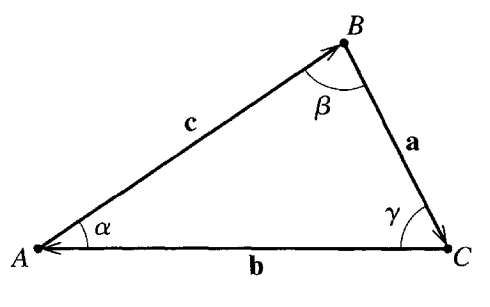
\includegraphics[keepaspectratio,alt={triangle}]{/Users/caballero/repos/teaching/modern-classical-mechanics/images/activities/1.15-triangle.png}}
\caption{triangle}
\end{figure}

\emph{(Figure: A triangle with sides \(\boldsymbol{a}\),
\(\boldsymbol{b}\), and \(\boldsymbol{c}\) and angles \(\alpha\),
\(\beta\), and \(\gamma\); reproduced from JRT.)}

\begin{itemize}
\item
  5a (5pt) Show that the area of the triangle can be given by any of
  these three equivalent expressions:
  \(A=\frac{1}{2}|\boldsymbol{a}\times\boldsymbol{b}|=\frac{1}{2}|\boldsymbol{b}\times\boldsymbol{c}|=\frac{1}{2}|\boldsymbol{c}\times\boldsymbol{a}|\).
\item
  5b (5pt) Use the equality of the three expressions for the area of the
  triangle to show that
  \(\frac{\sin{\alpha}}{a}=\frac{\sin{\beta}}{b}=\frac{\sin{\gamma}}{c}\),
  which is known as the
  \href{https://en.wikipedia.org/wiki/Law_of_sines}{Law of Sines}.
\end{itemize}

    \subsection{Exercise 6 (40pt), Numerical elements, getting started with
some simple
data}\label{exercise-6-40pt-numerical-elements-getting-started-with-some-simple-data}

\textbf{This exercise needs to be worked on in a Jupyter notebook, but
should be handed in as a PDF}. Remember to write your name(s).

Our first numerical attempt will involve reading data from file or just
setting up two vectors, one for position and one for time. Our data are
from

\href{https://youtube.com/watch?v=93dC0o2aHto}{\pandocbounded{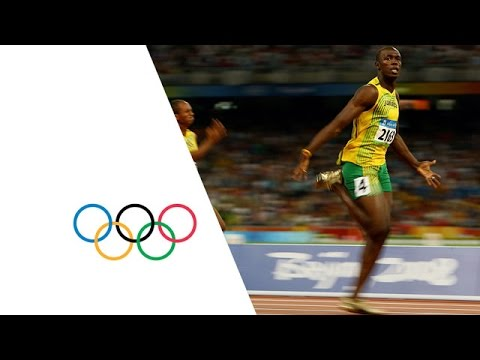
\includegraphics[keepaspectratio,alt={Usain Bolt's world record 100m during the olympic games in Beijing in 2008}]{/Users/caballero/repos/teaching/modern-classical-mechanics/images/activities/93dC0o2aHto.jpg}}}

\begin{itemize}
\tightlist
\item
  Direct Link:
  \href{https:curl//youtube.com/watch?v=93dC0o2aHto}{https://youtube.com/watch?v=93dC0o2aHto}
\end{itemize}

The data show the time used in units of 10m (see below). Before we
however venture into this, we need to repeat some basic Python syntax
with an emphasis on

\begin{itemize}
\item
  basic Python syntax for arrays
\item
  define and operate on vectors and matrices in Python
\item
  create plots for motion in 1D space
\end{itemize}

For more information, see
\href{https://dannycaballero.info/phy321msu/lecture-notes/chapter2.html\#python-practicalities-software-and-needed-installations}{this
link to Python support materials}. Here are some of the basic packages
we will be using this week

    \begin{tcolorbox}[breakable, size=fbox, boxrule=1pt, pad at break*=1mm,colback=cellbackground, colframe=cellborder]
\prompt{In}{incolor}{1}{\boxspacing}
\begin{Verbatim}[commandchars=\\\{\}]
\PY{o}{\PYZpc{}}\PY{k}{matplotlib} inline

\PY{k+kn}{import}\PY{+w}{ }\PY{n+nn}{numpy}\PY{+w}{ }\PY{k}{as}\PY{+w}{ }\PY{n+nn}{np} 
\PY{k+kn}{import}\PY{+w}{ }\PY{n+nn}{matplotlib}\PY{n+nn}{.}\PY{n+nn}{pyplot}\PY{+w}{ }\PY{k}{as}\PY{+w}{ }\PY{n+nn}{plt}
\PY{o}{\PYZpc{}}\PY{k}{matplotlib} inline
\end{Verbatim}
\end{tcolorbox}

    The first exercise here deals with simply getting familiar with vectors
and matrices.

We will be working with vectors and matrices to get you familiar with
them.

\begin{enumerate}
\def\labelenumi{\arabic{enumi}.}
\item
  Initalize two three-dimensional \(xyz\) vectors in the below cell
  using np.array({[}x,y,z{]}). Vectors are represented through arrays in
  python
\item
  V1 should have x1=1, y1 =2, and z1=3.
\item
  Vector 2 should have x2=4, y2=5, and z2=6.
\item
  Print both vectors to make sure your code is working properly.
\end{enumerate}

    \begin{tcolorbox}[breakable, size=fbox, boxrule=1pt, pad at break*=1mm,colback=cellbackground, colframe=cellborder]
\prompt{In}{incolor}{2}{\boxspacing}
\begin{Verbatim}[commandchars=\\\{\}]
\PY{n}{V1} \PY{o}{=} \PY{n}{np}\PY{o}{.}\PY{n}{array}\PY{p}{(}\PY{p}{[}\PY{l+m+mi}{1}\PY{p}{,}\PY{l+m+mi}{2}\PY{p}{,}\PY{l+m+mi}{3}\PY{p}{]}\PY{p}{)}
\PY{n}{V2} \PY{o}{=} \PY{n}{np}\PY{o}{.}\PY{n}{array}\PY{p}{(}\PY{p}{[}\PY{l+m+mi}{4}\PY{p}{,}\PY{l+m+mi}{5}\PY{p}{,}\PY{l+m+mi}{6}\PY{p}{]}\PY{p}{)}
\PY{n+nb}{print}\PY{p}{(}\PY{l+s+s2}{\PYZdq{}}\PY{l+s+s2}{V1: }\PY{l+s+s2}{\PYZdq{}}\PY{p}{,} \PY{n}{V1}\PY{p}{)}
\PY{n+nb}{print}\PY{p}{(}\PY{l+s+s2}{\PYZdq{}}\PY{l+s+s2}{V2: }\PY{l+s+s2}{\PYZdq{}}\PY{p}{,} \PY{n}{V2}\PY{p}{)}
\end{Verbatim}
\end{tcolorbox}

    \begin{Verbatim}[commandchars=\\\{\}]
V1:  [1 2 3]
V2:  [4 5 6]
    \end{Verbatim}

    If this is not too familiar, here's a useful link for creating vectors
in python
\url{https://docs.scipy.org/doc/numpy-1.13.0/user/basics.creation.html}.
Alternatively, look up the
\href{https://mhjensen.github.io/Physics321/doc/pub/week2/html/week2.html}{introductory
slides}.

Now let us do some basic mathematics with vectors.

Compute and print the following, and double check with your own paper
and pencil calculations:

\begin{itemize}
\item
  6a (2pt) Calculate \(\boldsymbol{V}_1-\boldsymbol{V}_2\).
\item
  6b (2pt) Calculate \(\boldsymbol{V}_2-\boldsymbol{V}_1\).
\item
  6c (2pt) Calculate the dot product
  \(\boldsymbol{V}_1\boldsymbol{V}_2\).
\item
  6d (2pt) Calculate the cross product
  \(\boldsymbol{V}_1\times\boldsymbol{V}_2\).
\end{itemize}

Here is some useful explanation on numpy array operations if you feel a
bit confused by what is happening, see
\url{https://www.pluralsight.com/guides/overview-basic-numpy-operations}.

The following code prints the first two exercises

    \begin{tcolorbox}[breakable, size=fbox, boxrule=1pt, pad at break*=1mm,colback=cellbackground, colframe=cellborder]
\prompt{In}{incolor}{3}{\boxspacing}
\begin{Verbatim}[commandchars=\\\{\}]
\PY{n+nb}{print}\PY{p}{(}\PY{n}{V1}\PY{o}{\PYZhy{}}\PY{n}{V2}\PY{p}{)}
\PY{n+nb}{print}\PY{p}{(}\PY{n}{V2}\PY{o}{\PYZhy{}}\PY{n}{V1}\PY{p}{)}
\end{Verbatim}
\end{tcolorbox}

    \begin{Verbatim}[commandchars=\\\{\}]
[-3 -3 -3]
[3 3 3]
    \end{Verbatim}

    For the dot product of V1 and V2 below we can use the \textbf{dot}
function of \textbf{numpy} as follows

    \begin{tcolorbox}[breakable, size=fbox, boxrule=1pt, pad at break*=1mm,colback=cellbackground, colframe=cellborder]
\prompt{In}{incolor}{4}{\boxspacing}
\begin{Verbatim}[commandchars=\\\{\}]
\PY{n+nb}{print}\PY{p}{(}\PY{n}{V1}\PY{o}{.}\PY{n}{dot}\PY{p}{(}\PY{n}{V2}\PY{p}{)}\PY{p}{)}
\end{Verbatim}
\end{tcolorbox}

    \begin{Verbatim}[commandchars=\\\{\}]
32
    \end{Verbatim}

    As a small challenge try to write your own function for the \textbf{dot}
product of two vectors.

Matrices can be created in a similar fashion in python. In this language
we can work with them through the package numpy (which we have already
imported)

    \begin{tcolorbox}[breakable, size=fbox, boxrule=1pt, pad at break*=1mm,colback=cellbackground, colframe=cellborder]
\prompt{In}{incolor}{5}{\boxspacing}
\begin{Verbatim}[commandchars=\\\{\}]
\PY{n}{M1} \PY{o}{=} \PY{n}{np}\PY{o}{.}\PY{n}{matrix}\PY{p}{(}\PY{p}{[}\PY{p}{[}\PY{l+m+mi}{1}\PY{p}{,}\PY{l+m+mi}{2}\PY{p}{,}\PY{l+m+mi}{3}\PY{p}{]}\PY{p}{,}
             \PY{p}{[}\PY{l+m+mi}{4}\PY{p}{,}\PY{l+m+mi}{5}\PY{p}{,}\PY{l+m+mi}{6}\PY{p}{]}\PY{p}{,}
             \PY{p}{[}\PY{l+m+mi}{7}\PY{p}{,}\PY{l+m+mi}{8}\PY{p}{,}\PY{l+m+mi}{9}\PY{p}{]}\PY{p}{]}\PY{p}{)}
\PY{n}{M2} \PY{o}{=} \PY{n}{np}\PY{o}{.}\PY{n}{matrix}\PY{p}{(}\PY{p}{[}\PY{p}{[}\PY{l+m+mi}{1}\PY{p}{,}\PY{l+m+mi}{2}\PY{p}{]}\PY{p}{,}
             \PY{p}{[}\PY{l+m+mi}{3}\PY{p}{,}\PY{l+m+mi}{4}\PY{p}{]}\PY{p}{,}
             \PY{p}{[}\PY{l+m+mi}{5}\PY{p}{,}\PY{l+m+mi}{6}\PY{p}{]}\PY{p}{]}\PY{p}{)}
\PY{n}{M3} \PY{o}{=} \PY{n}{np}\PY{o}{.}\PY{n}{matrix}\PY{p}{(}\PY{p}{[}\PY{p}{[}\PY{l+m+mi}{9}\PY{p}{,}\PY{l+m+mi}{8}\PY{p}{,}\PY{l+m+mi}{7}\PY{p}{]}\PY{p}{,}
             \PY{p}{[}\PY{l+m+mi}{4}\PY{p}{,}\PY{l+m+mi}{5}\PY{p}{,}\PY{l+m+mi}{6}\PY{p}{]}\PY{p}{,}
             \PY{p}{[}\PY{l+m+mi}{7}\PY{p}{,}\PY{l+m+mi}{6}\PY{p}{,}\PY{l+m+mi}{9}\PY{p}{]}\PY{p}{]}\PY{p}{)}
\end{Verbatim}
\end{tcolorbox}

    Matrices can be added in the same way vectors are added in python as
shown here

    \begin{tcolorbox}[breakable, size=fbox, boxrule=1pt, pad at break*=1mm,colback=cellbackground, colframe=cellborder]
\prompt{In}{incolor}{6}{\boxspacing}
\begin{Verbatim}[commandchars=\\\{\}]
\PY{n+nb}{print}\PY{p}{(}\PY{l+s+s2}{\PYZdq{}}\PY{l+s+s2}{M1+M3: }\PY{l+s+s2}{\PYZdq{}}\PY{p}{,} \PY{n}{M1}\PY{o}{+}\PY{n}{M3}\PY{p}{)}
\end{Verbatim}
\end{tcolorbox}

    \begin{Verbatim}[commandchars=\\\{\}]
M1+M3:  [[10 10 10]
 [ 8 10 12]
 [14 14 18]]
    \end{Verbatim}

    What happens if we try to do \(M1+M2\)?

That's enough vectors and matrices for now. Let's move on to some
physics problems!

We can opt for two different ways of handling the data. The data are
listed in the table here and represents the total time Usain Bolt used
in steps of 10 meters of distance. The label \(i\) is just a counter and
we start from zero since Python arrays are by default set from zero. The
variable \(t\) is time in seconds and \(x\) is the position in meters.
You may find it useful to include results at time \(t=0\) as well. The
position is obviously then \(x=0\) m.

i

0

1

2

3

4

5

6

7

8

9

x{[}m{]}

10

20

30

40

50

60

70

80

90

100

t{[}s{]}

1.85

2.87

3.78

4.65

5.50

6.32

7.14

7.96

8.79

9.69

\begin{itemize}
\tightlist
\item
  6e (6pt) You can make a file with the above data and read them in and
  set up two vectors, one for time and one for position. Alternatively,
  you can just set up these two vectors directly and define two vectors
  in your Python code.
\end{itemize}

The following example code may help here

    \begin{tcolorbox}[breakable, size=fbox, boxrule=1pt, pad at break*=1mm,colback=cellbackground, colframe=cellborder]
\prompt{In}{incolor}{7}{\boxspacing}
\begin{Verbatim}[commandchars=\\\{\}]
\PY{c+c1}{\PYZsh{} we just initialize time and position}
\PY{n}{x} \PY{o}{=} \PY{n}{np}\PY{o}{.}\PY{n}{array}\PY{p}{(}\PY{p}{[}\PY{l+m+mf}{10.0}\PY{p}{,} \PY{l+m+mf}{20.0}\PY{p}{,} \PY{l+m+mf}{30.0}\PY{p}{,} \PY{l+m+mf}{40.0}\PY{p}{,} \PY{l+m+mf}{50.0}\PY{p}{,} \PY{l+m+mf}{60.0}\PY{p}{,} \PY{l+m+mf}{70.0}\PY{p}{,} \PY{l+m+mf}{80.0}\PY{p}{,} \PY{l+m+mf}{90.0}\PY{p}{,} \PY{l+m+mf}{100.0}\PY{p}{]}\PY{p}{)}
\PY{n}{t} \PY{o}{=} \PY{n}{np}\PY{o}{.}\PY{n}{array}\PY{p}{(}\PY{p}{[}\PY{l+m+mf}{1.85}\PY{p}{,} \PY{l+m+mf}{2.87}\PY{p}{,} \PY{l+m+mf}{3.78}\PY{p}{,} \PY{l+m+mf}{4.65}\PY{p}{,} \PY{l+m+mf}{5.50}\PY{p}{,} \PY{l+m+mf}{6.32}\PY{p}{,} \PY{l+m+mf}{7.14}\PY{p}{,} \PY{l+m+mf}{7.96}\PY{p}{,} \PY{l+m+mf}{8.79}\PY{p}{,} \PY{l+m+mf}{9.69}\PY{p}{]}\PY{p}{)}
\PY{n}{plt}\PY{o}{.}\PY{n}{plot}\PY{p}{(}\PY{n}{t}\PY{p}{,}\PY{n}{x}\PY{p}{,} \PY{n}{color}\PY{o}{=}\PY{l+s+s1}{\PYZsq{}}\PY{l+s+s1}{black}\PY{l+s+s1}{\PYZsq{}}\PY{p}{)}
\PY{n}{plt}\PY{o}{.}\PY{n}{xlabel}\PY{p}{(}\PY{l+s+s2}{\PYZdq{}}\PY{l+s+s2}{Time t[s]}\PY{l+s+s2}{\PYZdq{}}\PY{p}{)}
\PY{n}{plt}\PY{o}{.}\PY{n}{ylabel}\PY{p}{(}\PY{l+s+s2}{\PYZdq{}}\PY{l+s+s2}{Position x[m]}\PY{l+s+s2}{\PYZdq{}}\PY{p}{)}
\PY{n}{plt}\PY{o}{.}\PY{n}{title}\PY{p}{(}\PY{l+s+s2}{\PYZdq{}}\PY{l+s+s2}{Usain Bolt}\PY{l+s+s2}{\PYZsq{}}\PY{l+s+s2}{s world record run}\PY{l+s+s2}{\PYZdq{}}\PY{p}{)}
\PY{n}{plt}\PY{o}{.}\PY{n}{show}\PY{p}{(}\PY{p}{)}
\end{Verbatim}
\end{tcolorbox}

    \begin{center}
    \adjustimage{max size={0.9\linewidth}{0.9\paperheight}}{hw1_files/hw1_20_0.png}
    \end{center}
    { \hspace*{\fill} \\}
    
    \begin{itemize}
\item
  6f (6pt) Plot the position as function of time
\item
  6g (10pt) Compute thereafter the mean velocity for every interval
  \(i\) and the total velocity (from \(i=0\) to the given interval
  \(i\)) for each interval and plot these two quantities as function of
  time. Comment your results.
\item
  6h (10pt) Finally, compute and plot the mean acceleration for each
  interval and the total acceleration. Again, comment your results. Can
  you see whether he slowed down during the last meters?
\end{itemize}


    % Add a bibliography block to the postdoc
    
    
    
\end{document}
